\documentclass[runningheads]{llncs}

\usepackage{graphicx}

\begin{document}

\title{My Cool Title}

\author{Jacobus C. Lock\inst{1} \and
  Gzegorz Cielniak\inst{1} \and
  Andrea Tramontano\inst{2} \and
  Nicola Bellotto\inst{1}
}
\authorrunning{J.C. Lock et. al.}
\institute{University of Lincoln, Lincoln, UK \and
  Universita Degli Studi Di Padova, Italy
}

\maketitle

\begin{abstract}
  Cool abstract here
  \keywords{All the best keywords}
\end{abstract}

\section{Introduction}

It is estimated that there are almost half a billion people today that live with mild to severe levels of vision impairments or total blindness and this number is expected to significantly rise with an ageing population~\cite{bourne2017magnitude}. There has been a rise interest from industrial partners in utilising modern technology to make their products more accessible and improvements in modern computing power and image processing capabilities have made this easier. The work we present here is part of the ActiVis project that aims to assist people with vision impairments (PwVI) to independently navigate and find objects within an unknown indoor environment using only a mobile phone and its camera. This system implements ideas from the active vision field~\cite{bajcsy2017,bellotto2013}, but replaces the electro-mechanical servo typically found in active vision systems, with a user's arm and hand as pictured in Fig.~\ref{fig:system-in-use}. This project expands upon concepts originally proposed in~\cite{bellotto2013} and~\cite{lock2017portable} and builds off of the system introduced in~\cite{lock2019active}.

\begin{figure}
  \centering
  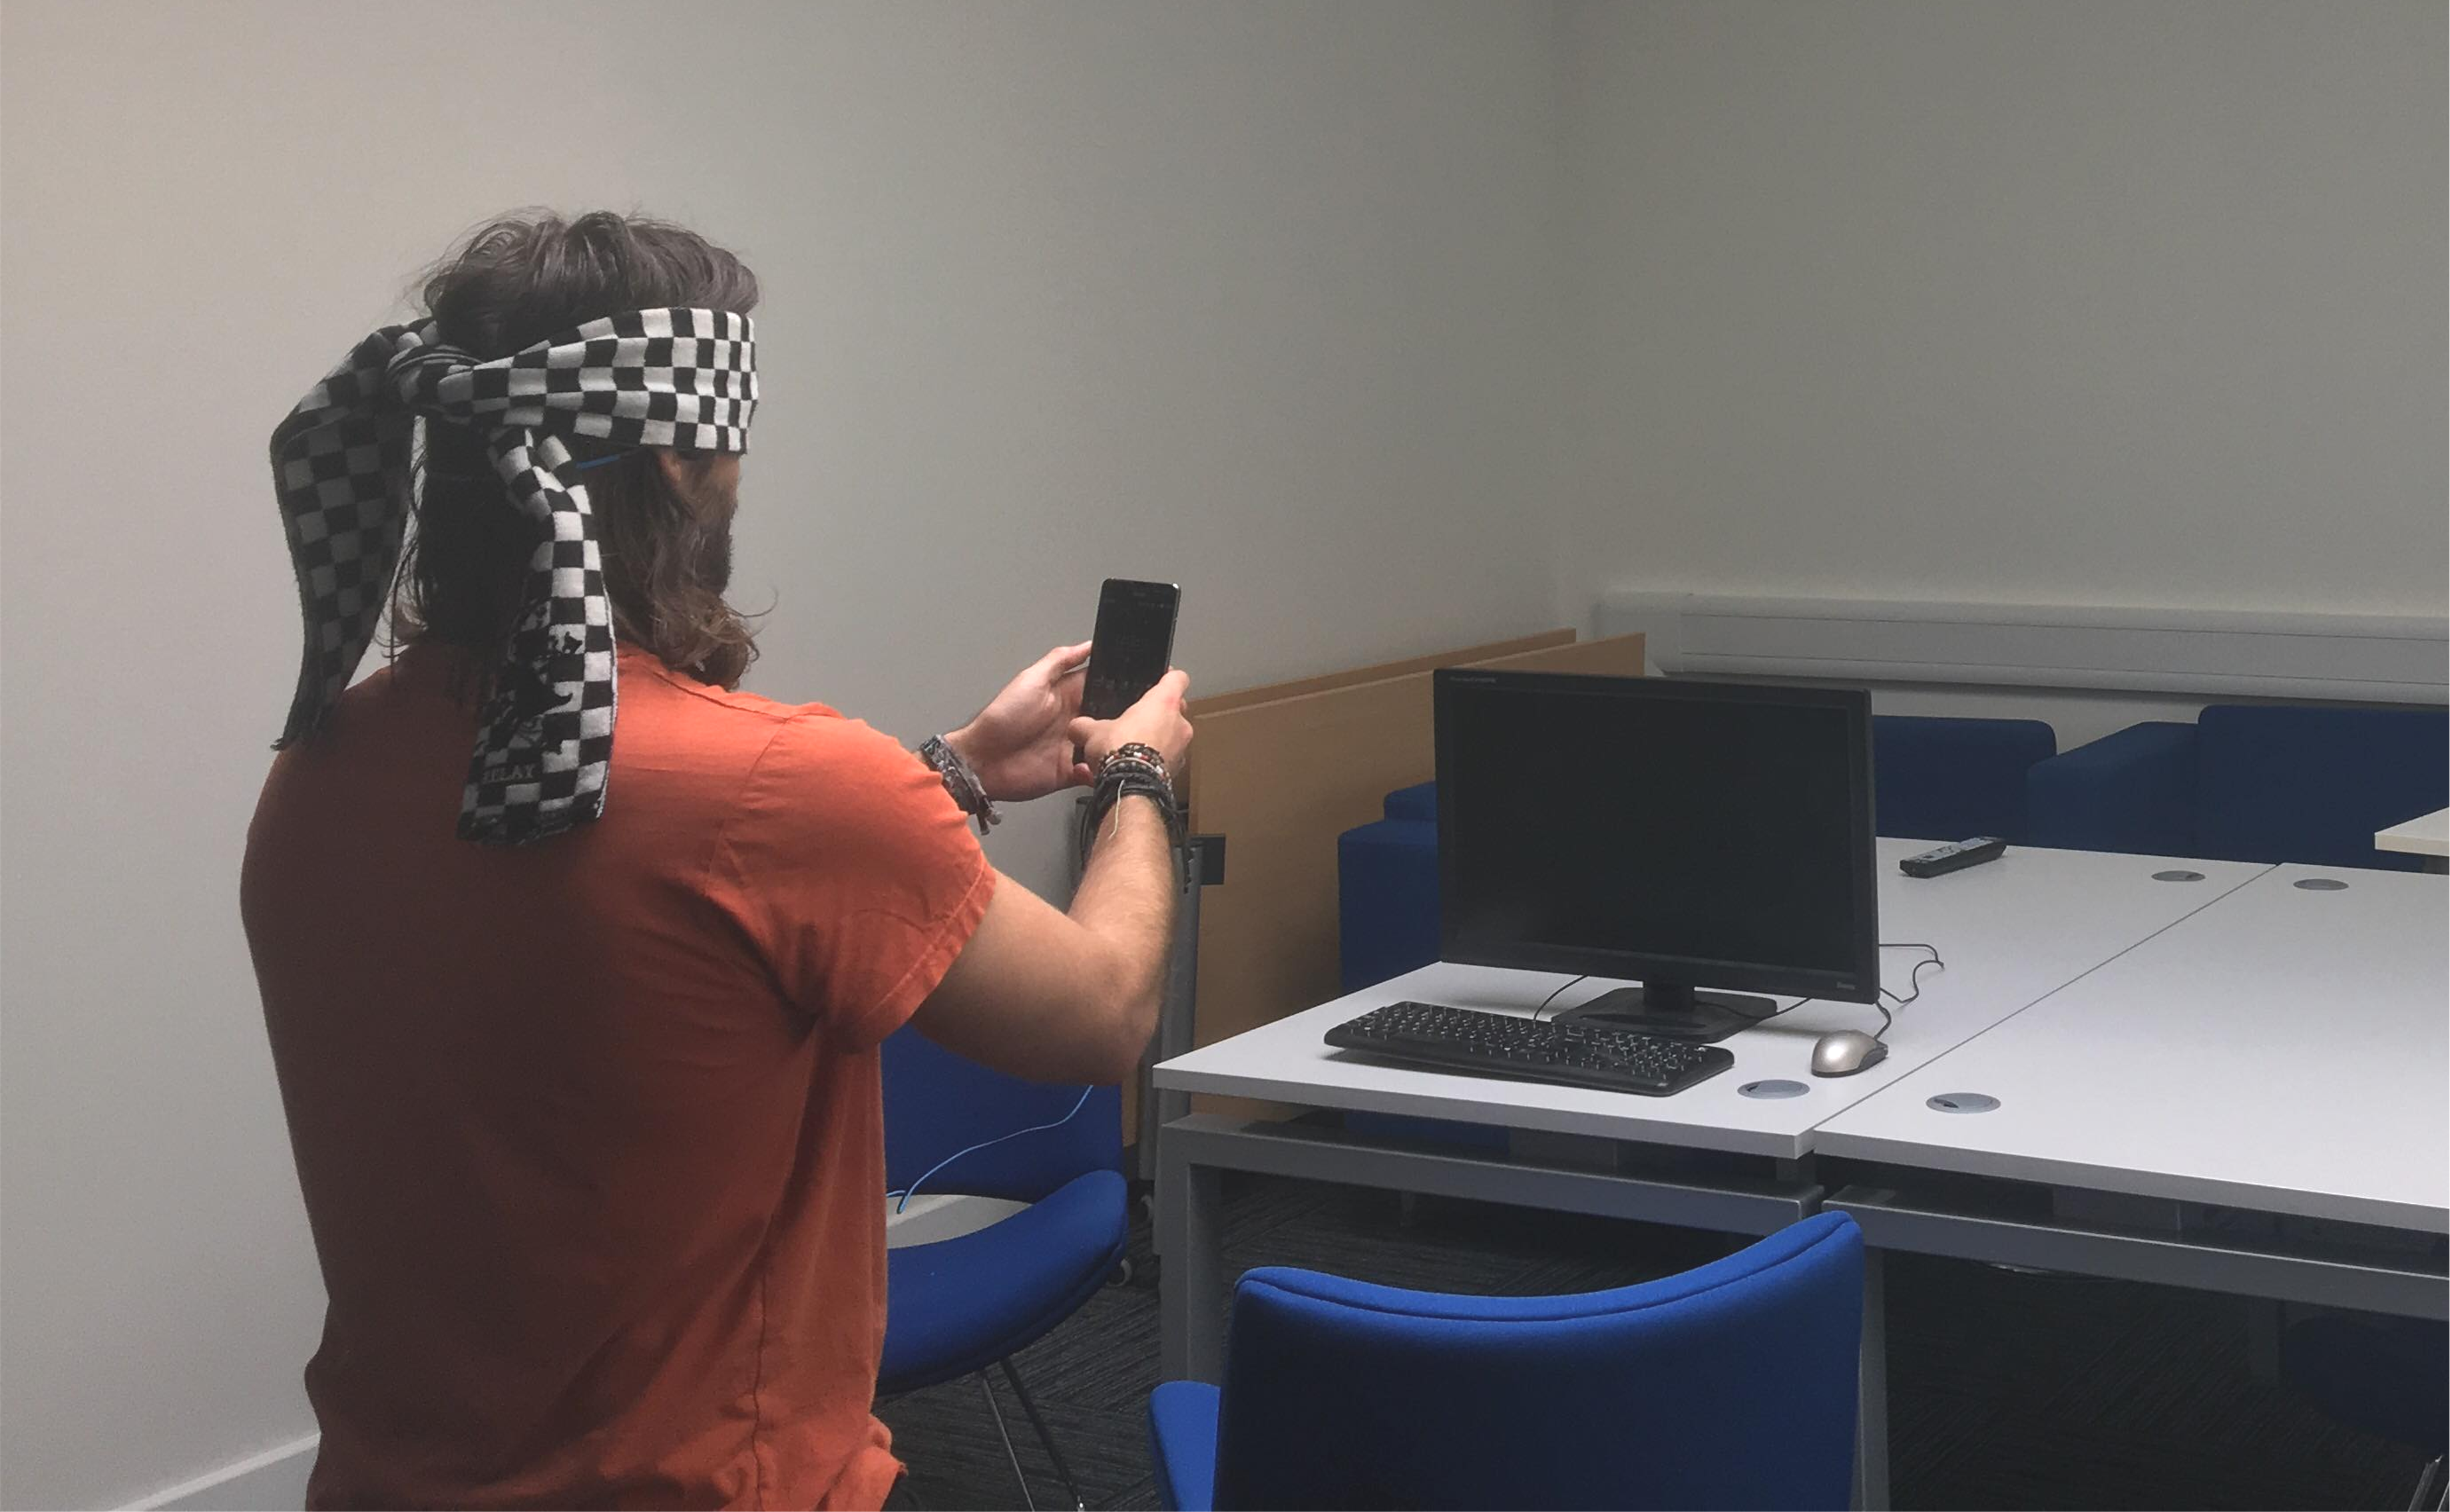
\includegraphics[width=0.38\textwidth]{figures/system_use.png}
  \caption{The system in use during an experiment. }\label{fig:system-in-use}
\end{figure}

\section{Previous Work}

\section{System Design}

\section{Experiment Design}

\section{Results}

\section{Conclusion}

\bibliographystyle{splncs04}
\bibliography{bib}

\end{document}
